\chapter{A Compiler for \textsc{x86/32}}

In this section, finally, we will consider a codegenerator for \textsc{x86/32} processor, the principal study
object of the whole course. In this particular chapter we will only deal with the simplest compiler for
straight-line programs, but as the source language evolves the native-code compiler will get more
and more features.

Of course the main question for now is what implementing a native-code compiler amounts to. Luckily, as we will
see shortly, this task is not much different from what we already can do. In order to turn our source program
into machine code we only need to convert it into a text in an \emph{assembly} language. Then we entrust
the \textsc{GCC} toolchain to make the rest of the work~--- compile this assembly program into object file,
link (multiple) compiled object files and some libraries into executable, etc. This approach is by no means
exotic~--- nowdays the majority of compilers are implemented exactly following this roadmap which makes it
possible to reuse all stages of compilation starting from object file generation by many compilers (and thus
avoid of making a lot of similar errors anew).

An important methodological difference of what we are going to do in this chapter is that we \emph{will not}
discuss the operational semantics of the assembly language. The motivation is that this language is very similar
in its generic features to stack machine language, which we already dealt with. As we generate native code from
stack machine, the compiler assumed to be very simple, and its formal description is expected to be superfluous.
On the other hand there are a lot of tiny simple details in machine architecture which would make formal description
boring and cumbersome, so we better discuss them in informal terms. But this does not mean that assembly languages c
annot be properly described in formal terms, and there are lots of witnesses of the opposite.

\section{Hardware Architecture}

In this section we consider some basic principles of digital hardware organization, describe how actual hardware works,
what components it is comprised of, and how it interprets machine program. All these subjects are topics of interest
for the field of \emph{hardware architecture}; we only scratch the surface of this very interesting and important
domain to the minimal extent needed to understand the essence of computations performed on actual hardware.

\begin{figure}[t]
  \centering
  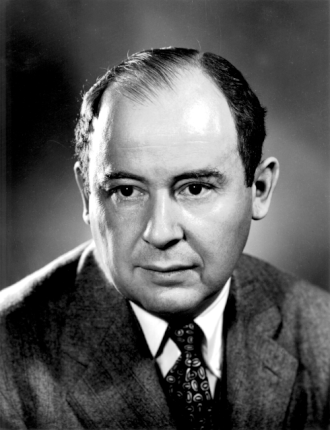
\includegraphics[scale=0.5]{images/JohnvonNeumann.png}
  \caption{John von Neumann}
\end{figure}

From a birds-eye view a hardware computer consists of \emph{memory}, \emph{central processor unit} (CPU), and
\emph{input-output} subsystem. This very general decomposition is known under the name ``von Neumann architecture'' named
after John von Neumann. In von Neumann architecture programs are kept in the same memory as data; this is
sometimes contrasted to so-called \emph{Harvard architecture} where a separate memory is dedicated solely to
keep programs. While the majority of general-purpose computers follow von Neumann architecture the Harvard one can be
found in some embedded devices. The real implementations of both approaches, of course, are much more complicated then
the generic scheme: there can be more than one CPU core, the CPU core itself contains one or more \emph{arithmetic-logic units} (ALU) and
\emph{multiplexers} (MUX) to perform conditional computations, memory subsystem is implemented using \emph{memory controller} and can
incorporate one or more levels of \emph{cache}, there is, as a rule, a separate subsystems to handle software and hardware \emph{interrupts},
support \emph{virtual memory}, \emph{virtualization}, etc. However, the general construct of a \emph{hardwired electronic interpreter}
of programs represented as sequences of bits kept in memory can be easily discovered in all digital programmable devices. This is,
by the way, justifies the central role of the concept of interpreter: there is actually no way to evaluate a program other than
to run it on some (perhaps, hardware) interpreter.

An important observation is that not all details of hardware organization are visible at the application level; some of them are intentionally
designed to be completely transparent to an end-user application. For example, hardware interrupts, virtual memory, cache, etc., as a rule are
invisible for a regular application, which means that a compiler in the \emph{majority of cases} (but not always!) can ignore the presence of
these subsystems. Moreover, a compiler as a rule does not deal with a certain part of hardware functionality and instruction set just
because the source language does not have corresponding abstractions. Finally, as a regular interpreter can be implemented in
various ways even using the same implementation language, hardware platforms also can have different implementations while sharing
the same ``surface'' architecture and instruction set. This surface, or \emph{macroarchitecture} of \textsc{x86/32} is a subject
of our close attention in this chapter. But, first, we consider the very principles digital programmable hardware is based on.

\subsection{Principles of Digital Hardware Organization}

Digital hardware in the vast majority of versions operates on \emph{binary} data. In this form all sorts of data a computer
deals with is represented as sequences of integer numbers in binary representation, i.e. in a regular positional
encoding radix 2; we assume the reader's familiarity with this construct. The advantage of this representation
is that it only requires from a physical system representing one digit to be in one of two stable states. In real
hardware these two states (0 and 1) are usually represented as different voltage levels measured against some
baseline (ground).





\section{Code Generation with Symbolic Interpreter}

\section{}


